%Project Narrative
\documentclass[11pt]{article}
\usepackage[margin=1in]{geometry}
\usepackage{color}
\usepackage{graphicx}
\usepackage{url}
\usepackage{multicol}
\usepackage{wrapfig}
\usepackage{amsmath}
\usepackage{amssymb}
\usepackage{caption}
\usepackage{subcaption}
\usepackage[round]{natbib}
\bibpunct[; ]{[}{]}{,}{n}{}{;} 
\bibliographystyle{abbrvnat}
\setcitestyle{authoryear,open={(},close={)}}
\usepackage[usenames,dvipsnames,svgnames,table]{xcolor}
\usepackage[innercaption]{sidecap} % side captions
\sidecaptionvpos{figure}{c}

\begin{document}

\title{\vspace{-5ex}Research Approach: Evolutionary genetics of maize\vspace{-4ex}}
\author{}
\date{}
\maketitle


%Research Approach - not to exceed 1,500 words - of your ongoing and planned research program.
%May include a list of essential references and up to one page of figures.
%Figures and accompanying short legends may be interleaved with the body of the research approach text.
%Figures, legends, and essential references are not included in the 1,500 word limit.

\section*{Maize as a model for plant evolutionary genetics}

Genome size variation in plants, humans. 
Differences in large complex genomes -- Fraser \citep{fraser2013gene} vs. \citep{pyhajarvi2013complex} or \citep{hancock2011adaptation} and gene expression \citep{hufford2012comparative}



\section*{Domestication}



\begin{figure*}[tb]
%\vspace*{.05in}
\centering
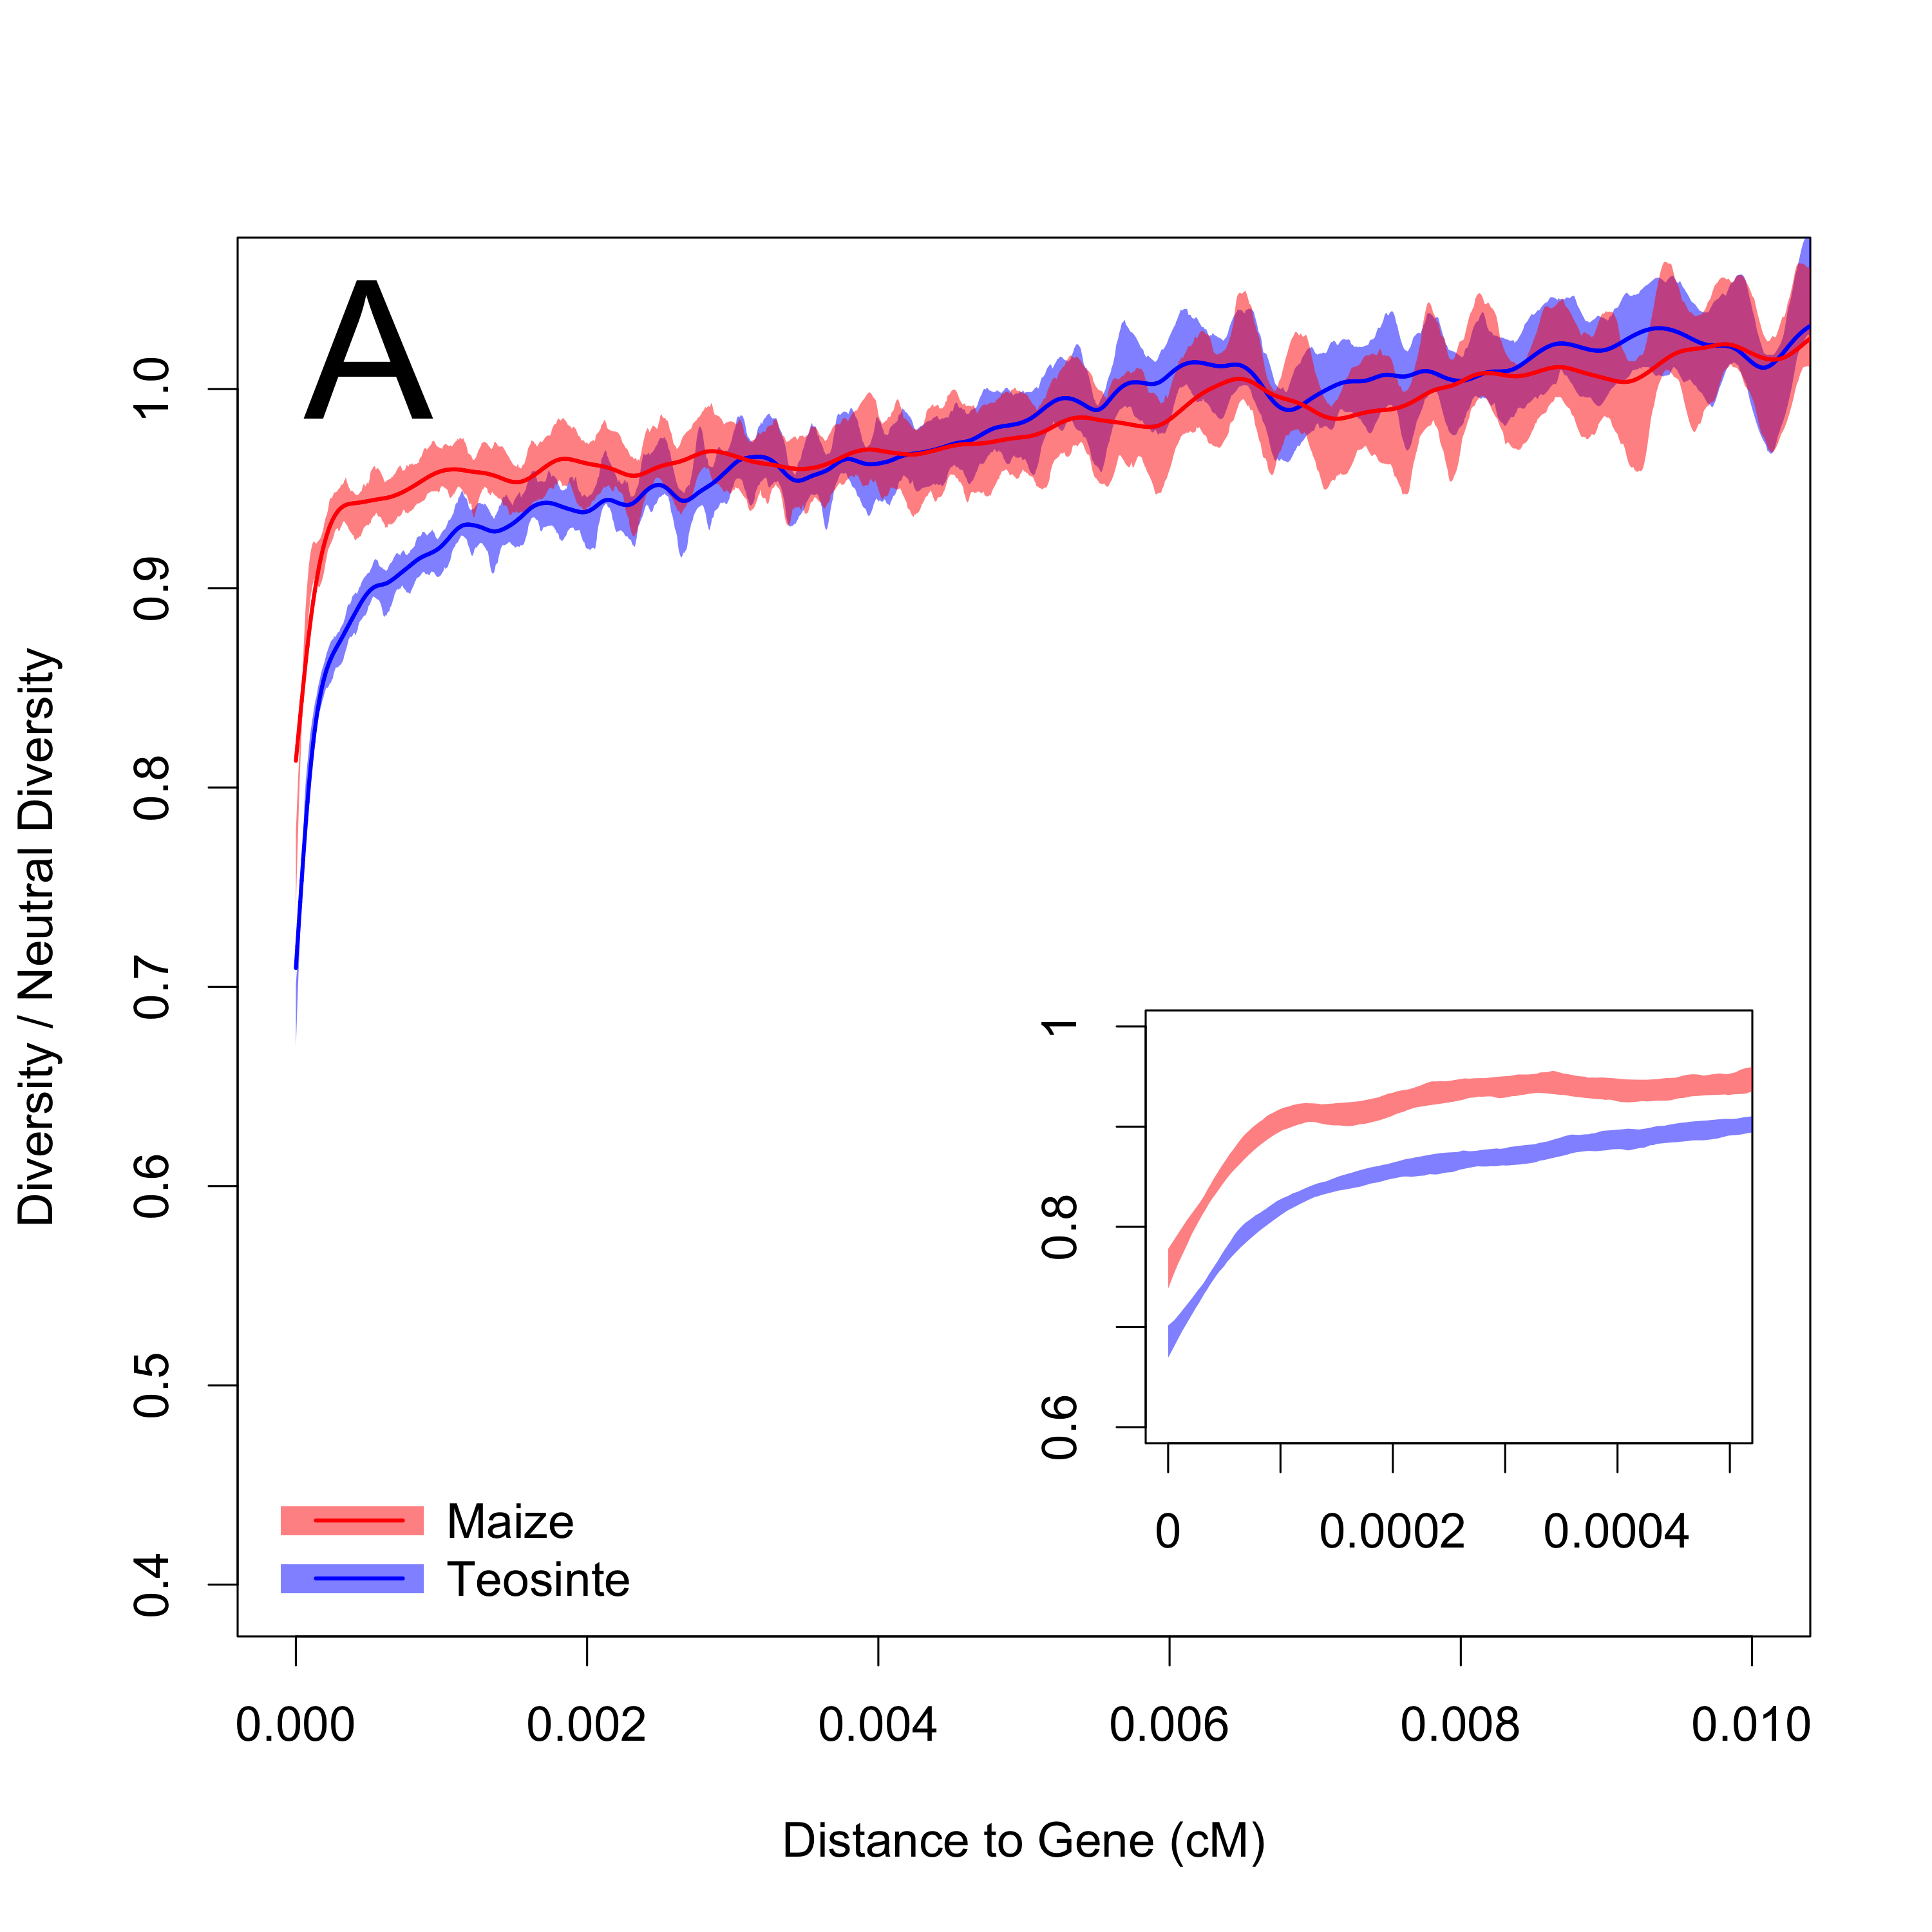
\includegraphics[width=.45\textwidth]{figs/distanceToGene_WithSignificance_Folded2_manuscript.png} 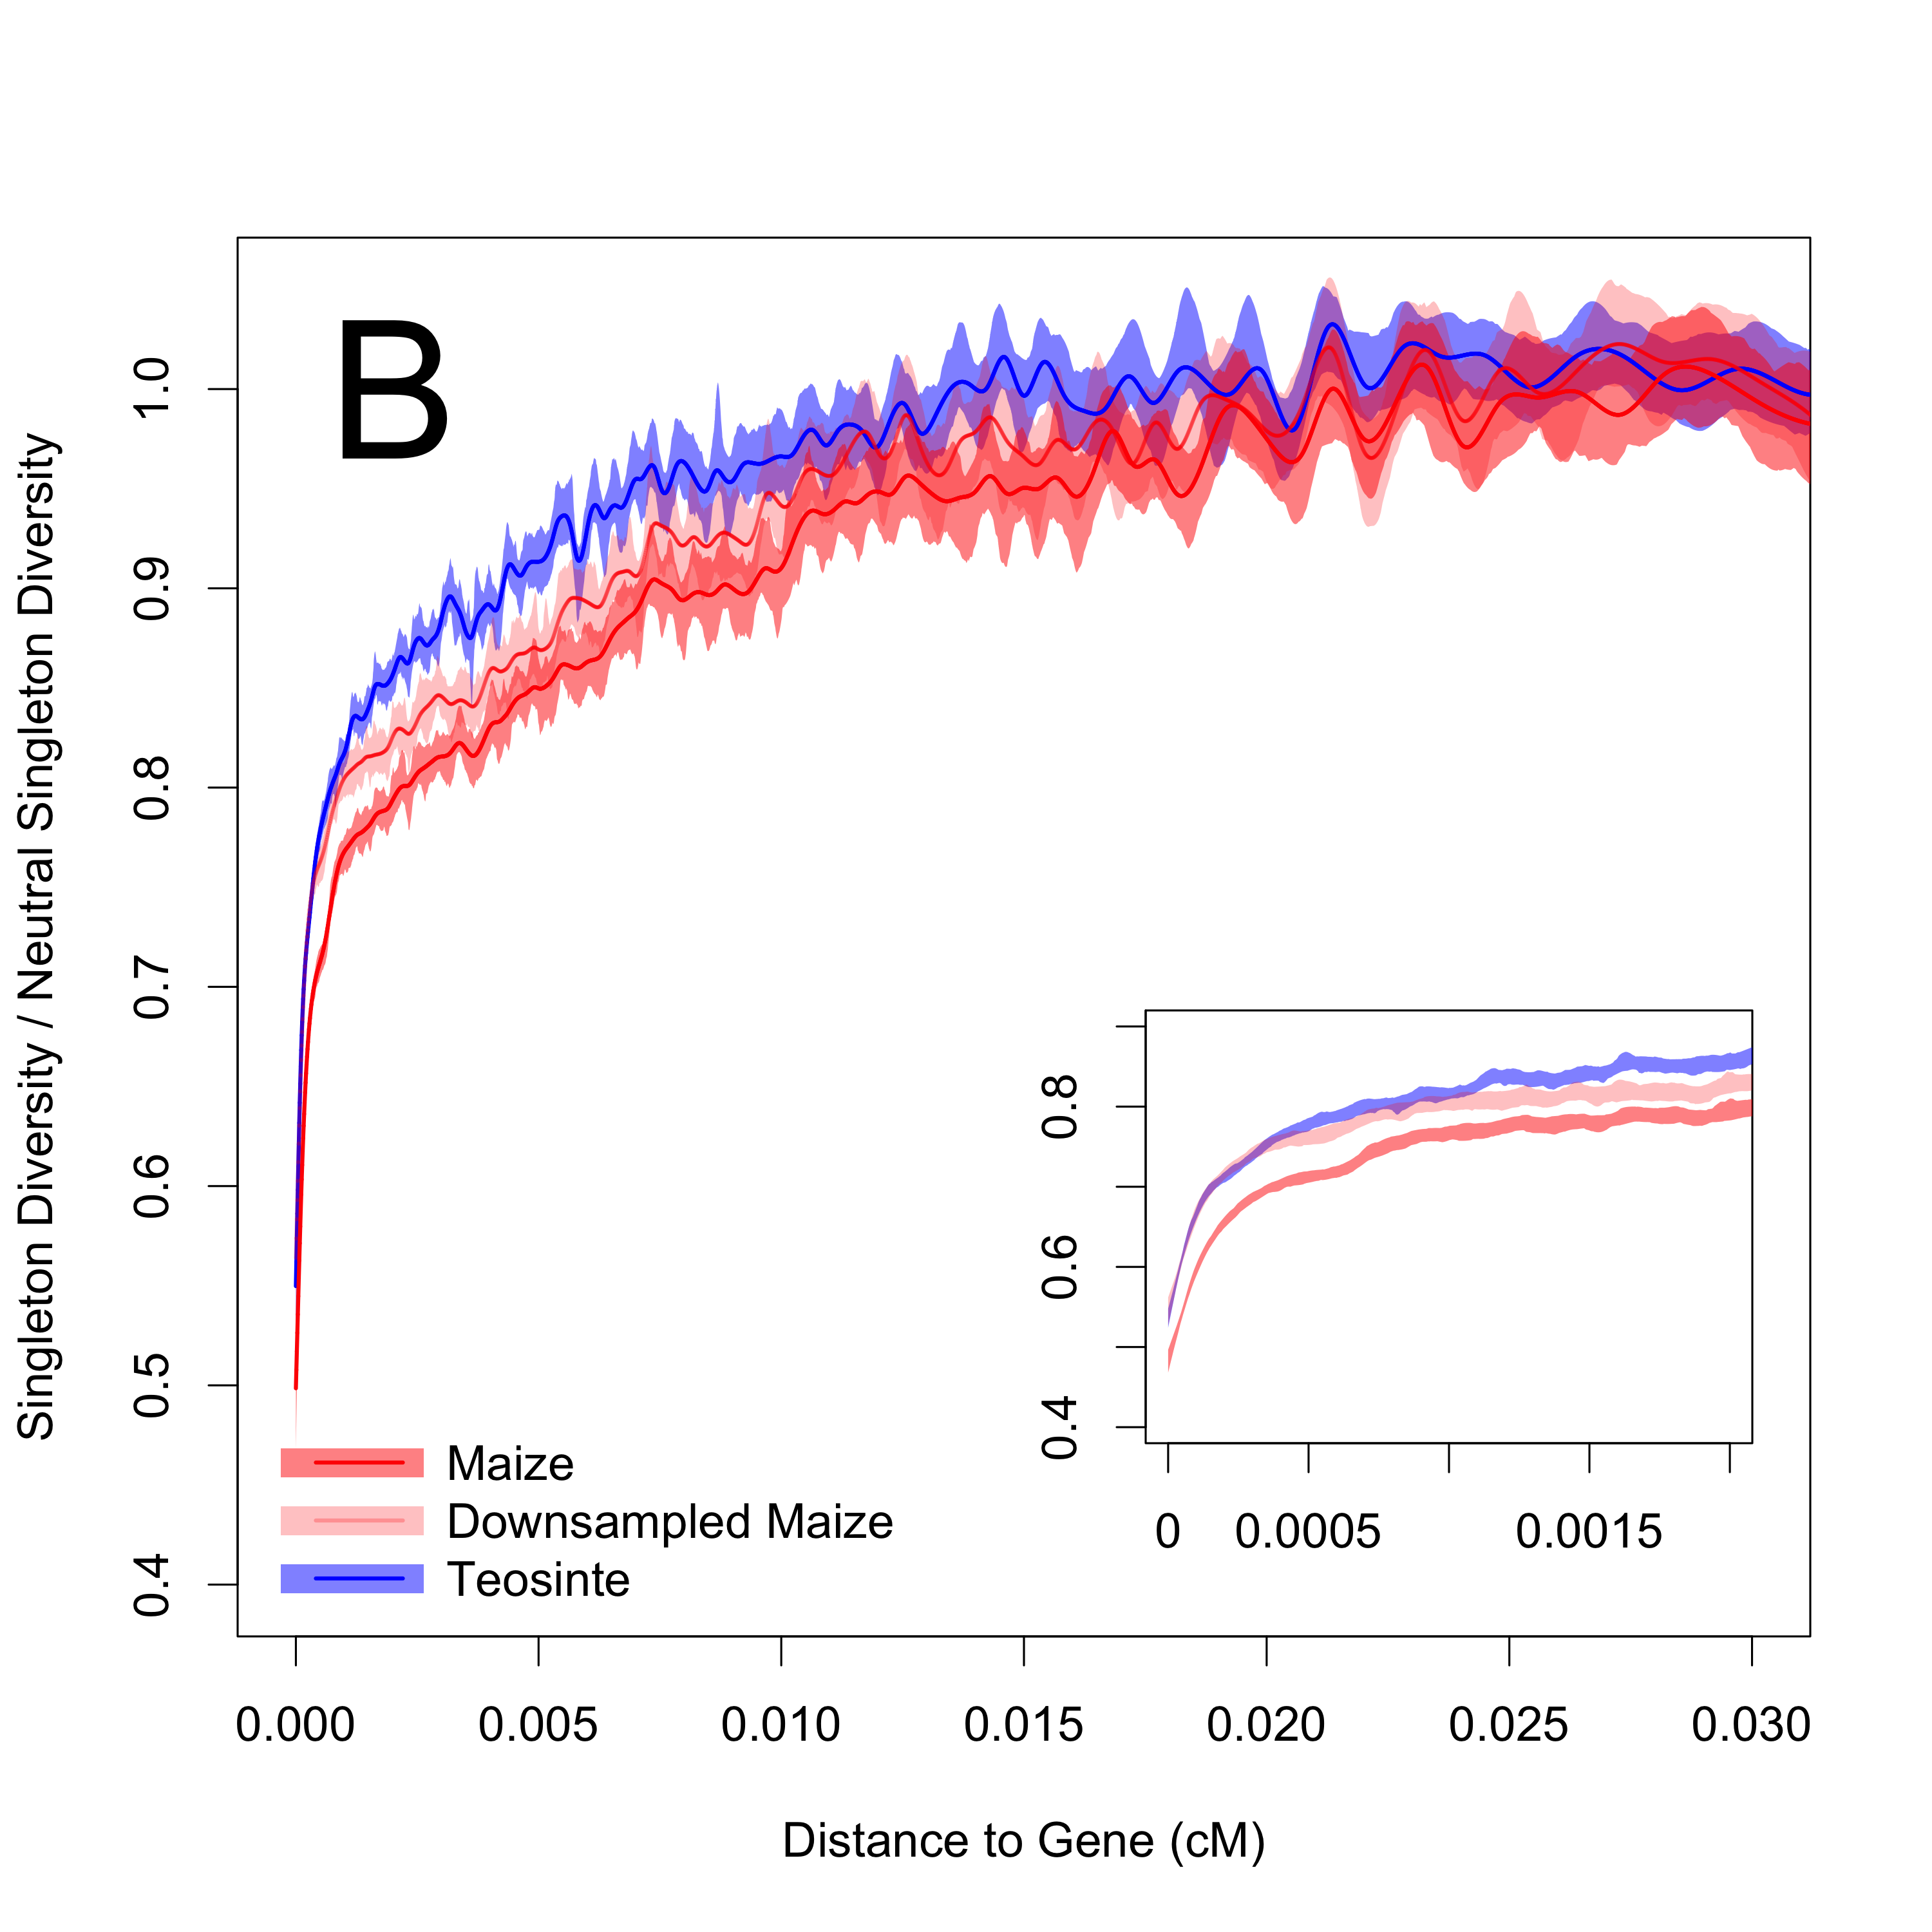
\includegraphics[width=.45\textwidth]{figs/distanceToGene_WithSignificance_Singletons_Downsampled_threeLines_manuscript.png}
\caption{Relative level of diversity versus distance to the nearest
  gene, in maize and teosinte. Two measures of diversity are shown. \textbf{A} Pairwise
  nculeotide diversity $\pi$ is most influenced by intermediate frequency
  alleles and reflective of long-term evolutionary patterns. The weaker effect of purifying selection seen in maize is consistent with a domestication bottleneck that lowered long-term effective population size. 
  \textbf{B} Number of singletons polymorphisms $\eta_1$. These lowest frequency alleles are young, reflecting very recent evolutionary patterns. Here the impact of purifying selection is stronger in maize, consistent with exponential growth following domestication. \label{fig:purify}}
\end{figure*}
%tim figure

\section*{Local adaptation}
% architecture, biotic interactions, climate, introgression

%figure from hufford

\section*{Experimental evolution}

\begin{figure*}[tb]   
  \begin{center}
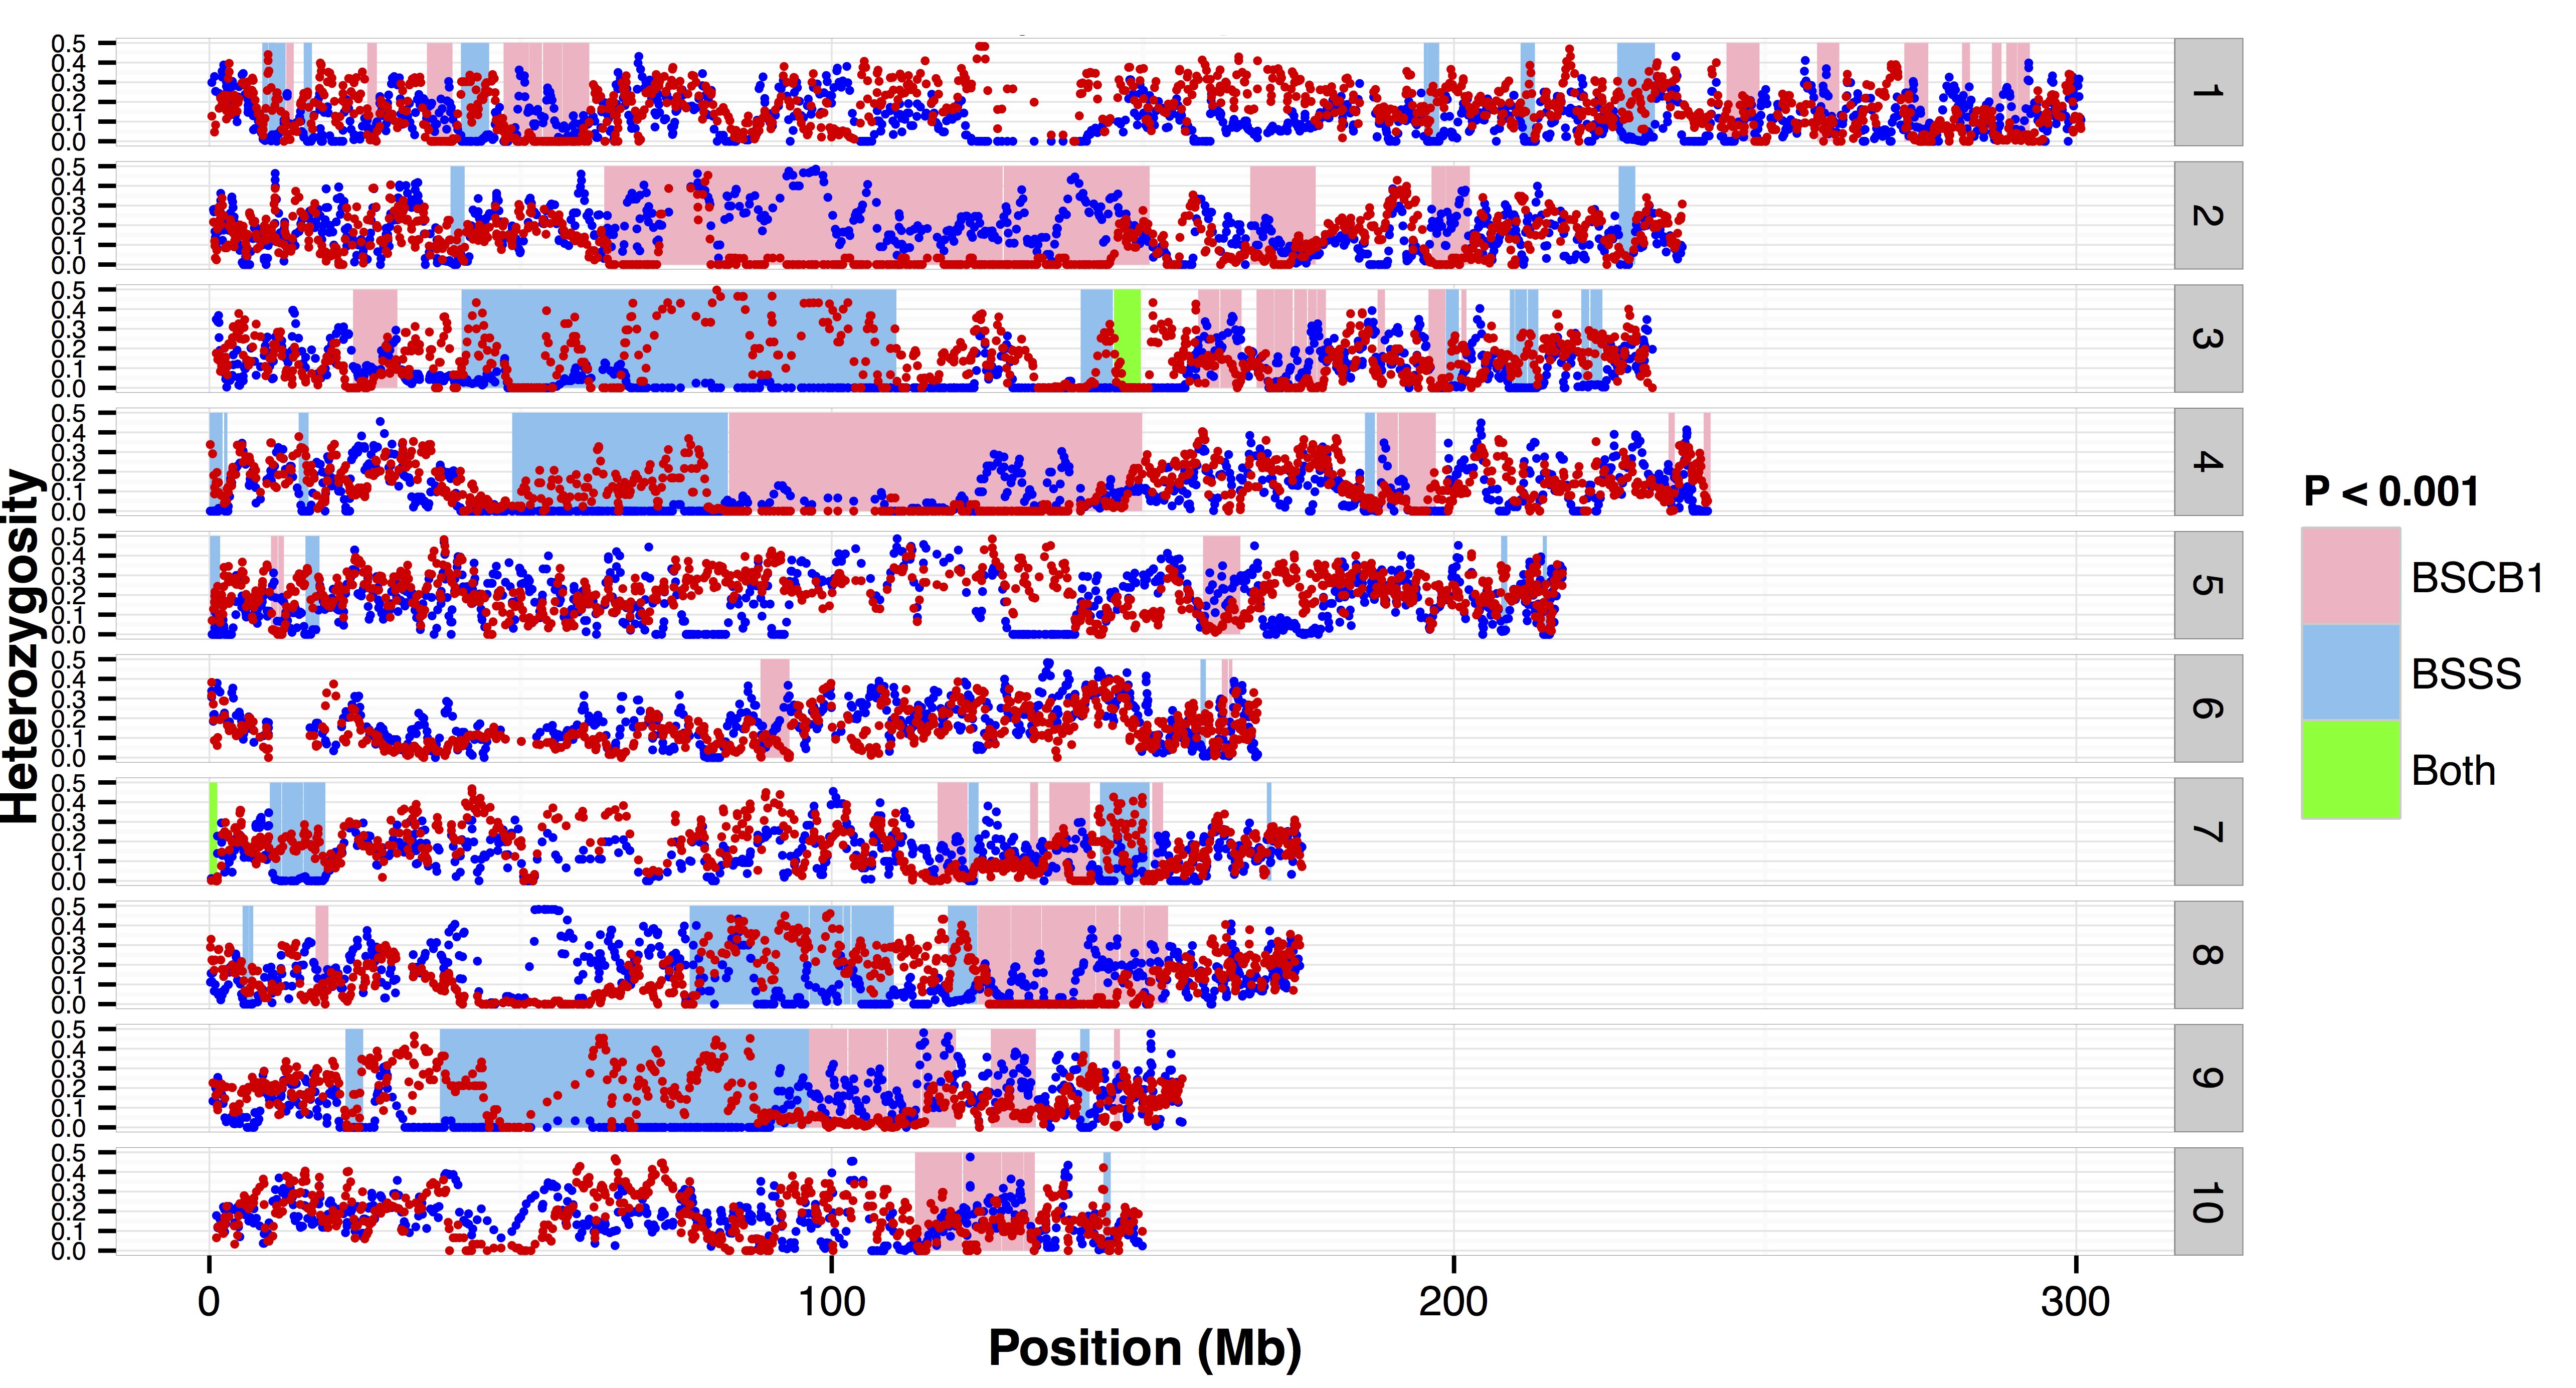
\includegraphics[width=0.8\linewidth]{figs/gerke.png}
   \caption{Heterozygosity across all 10 chromosomes of maize from cycle 16 of the Iowa Reciprocal Recurrent Selection experiment. Heterozygosity values in the BSSS  (blue dots) and BSCB1 (red dots) populations are superimposed in one panel. 2cM windows of heterozygosity lower than 10 of 10,000 simulations ($P<0.001$) are shaded in light blue (BSSS) or pink (BSCB1). Two regions genome-wide show significantly low heterozygosity in both populations and are shaded green.} 
    \label{fig:heterotic}
  \end{center}
\end{figure*}

\section*{Genome evolution}

TE insertions \citep{studer2011identification, makarevitch2015transposable} and regulation. 
genome size too \citep{tenaillon2011genome}

michelle stats. 344K insertions

TEs, CNVs, genome size evolution

missing data vs. allele frequencies.
TEs
\begin{figure*}[tb]
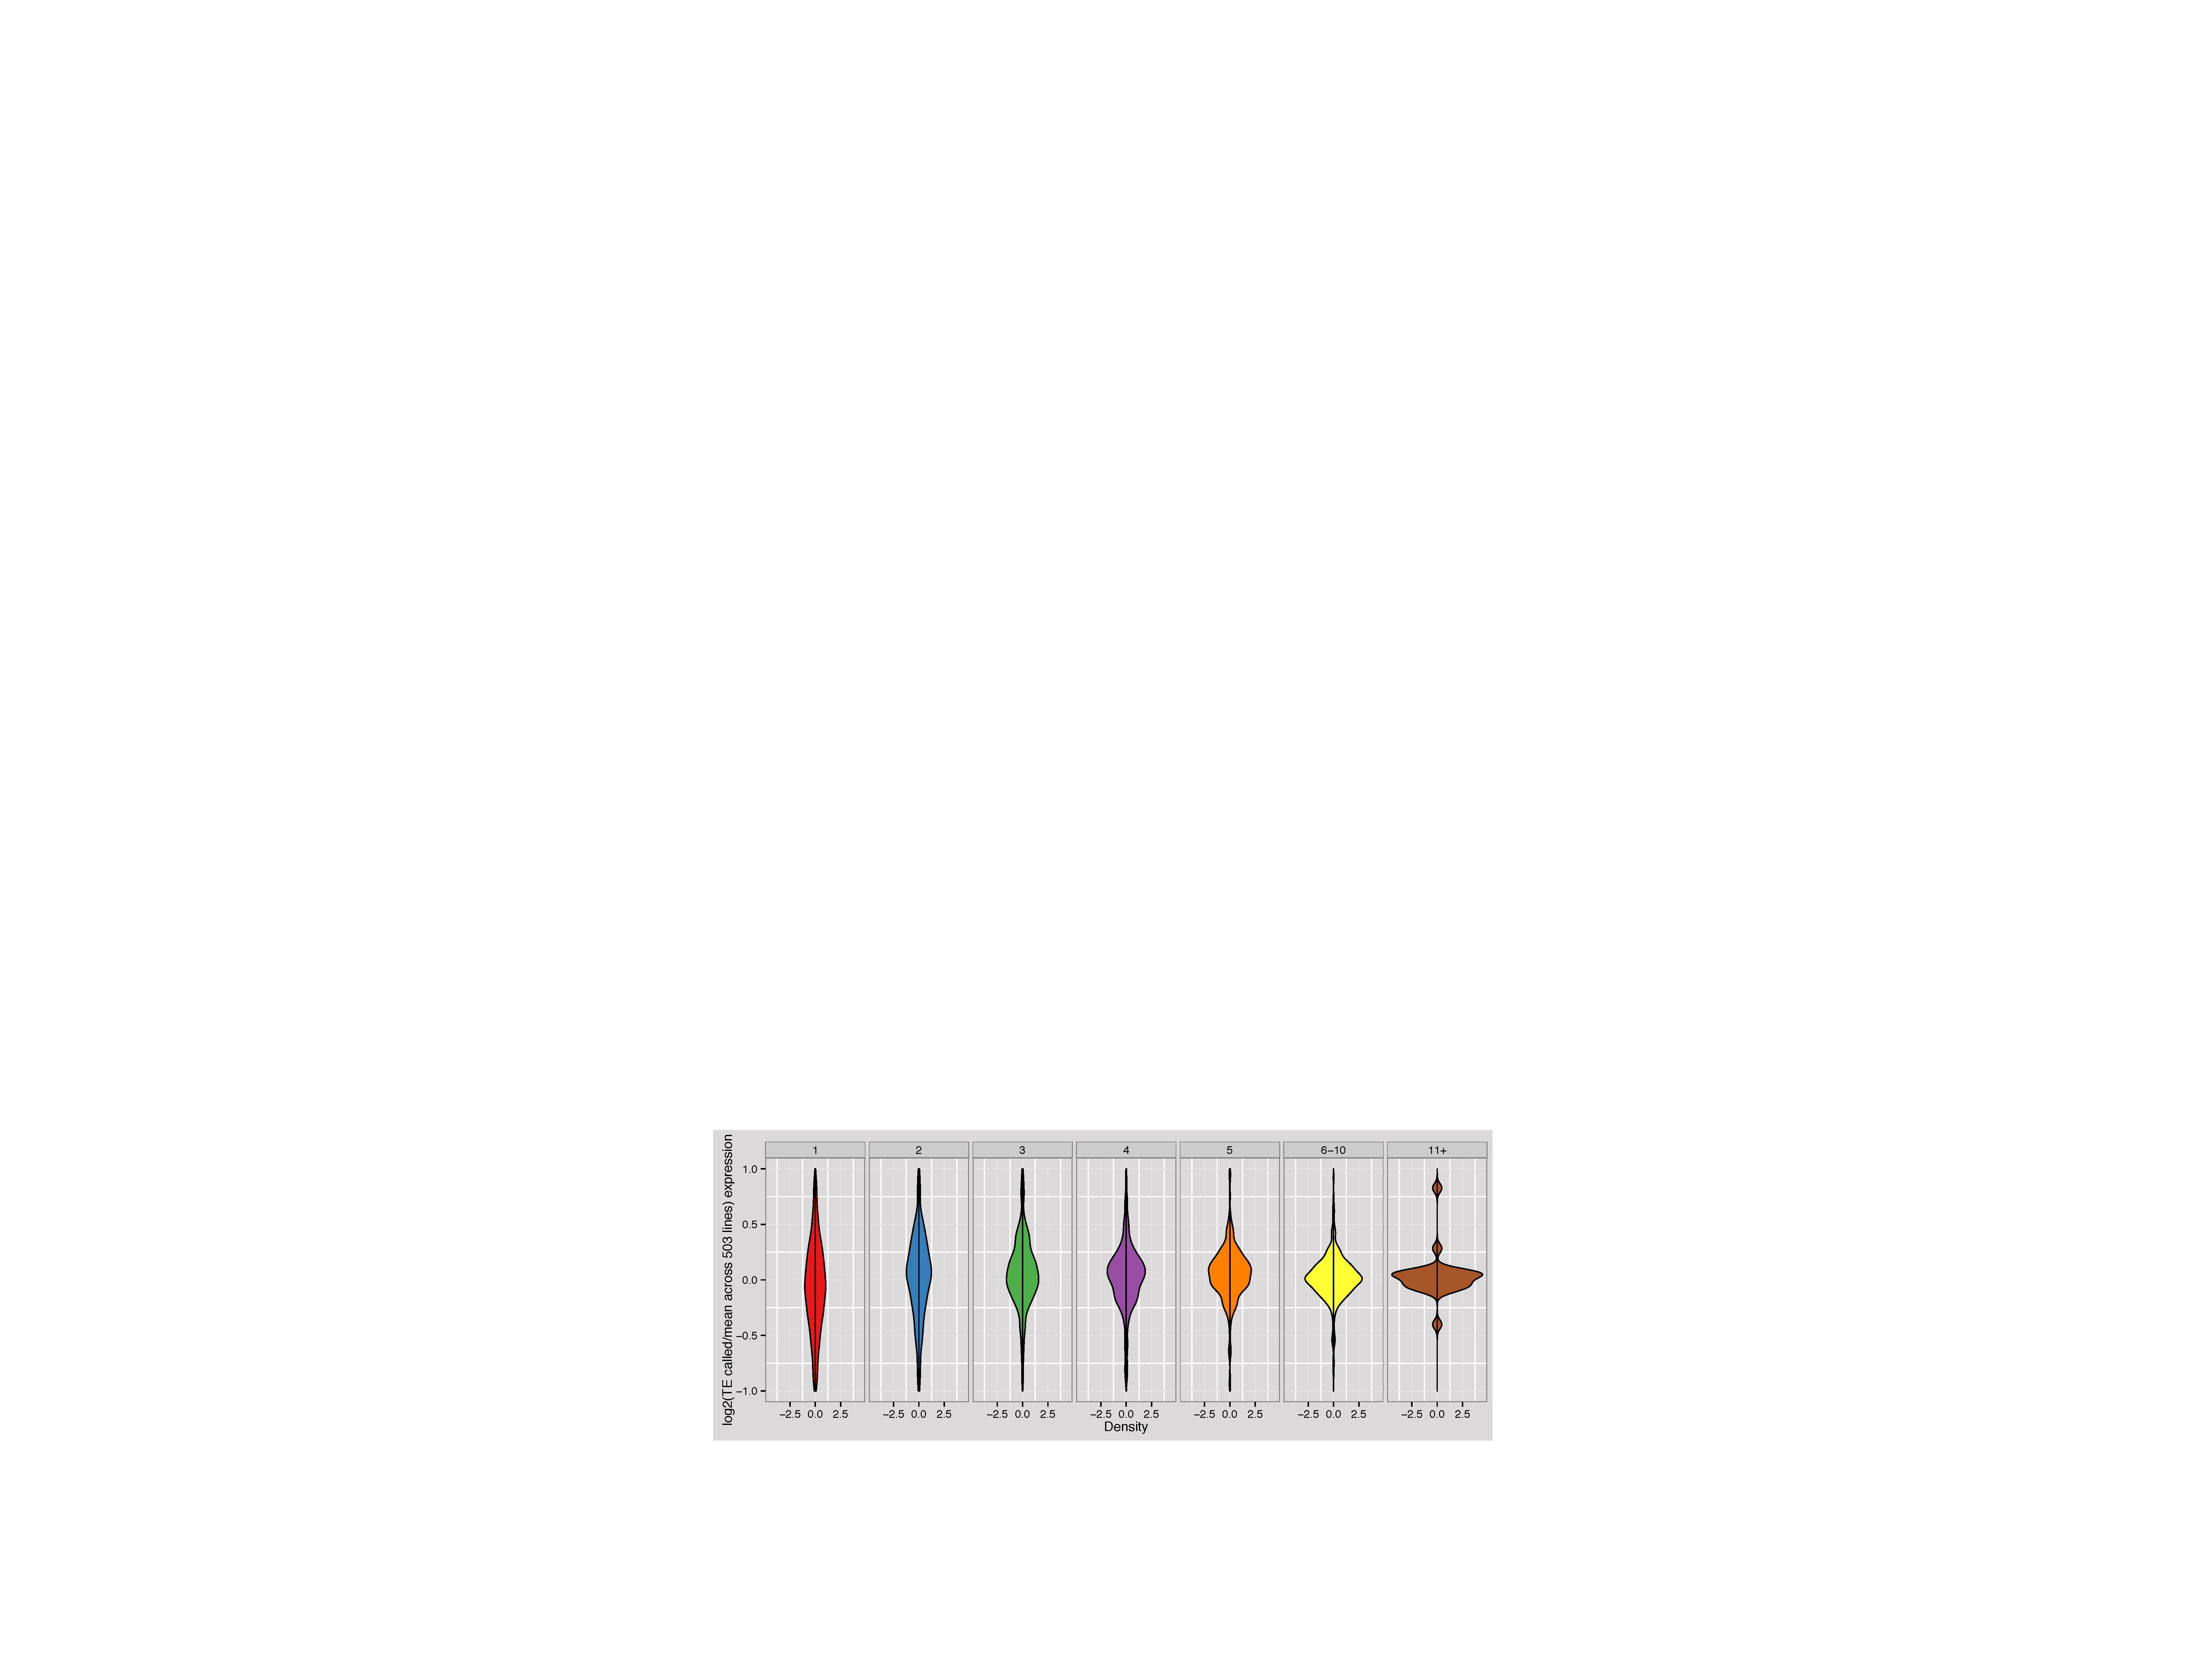
\includegraphics[width=0.45\linewidth]{figs/te_expression.pdf}
\caption{The effect of \emph{de novo} non-reference transposable element insertion on gene expression. Panels show the impact of insertions identified in 1 (far left) to $>10$ (far right) inbred lines in a panel of 23 maize inbreds.  Shown in each panel is the relative expression of genes in inbred lines with the insertion within the annotated gene region to the mean expression of that gene across 500 maize lines \citep{hirsch2014insights}. Recent, low frequency insertions tend to decrease gene expression compared to older, high-frequency insertions.  } 
\label{fig:te_expression}
\end{figure*}

\begin{SCfigure}
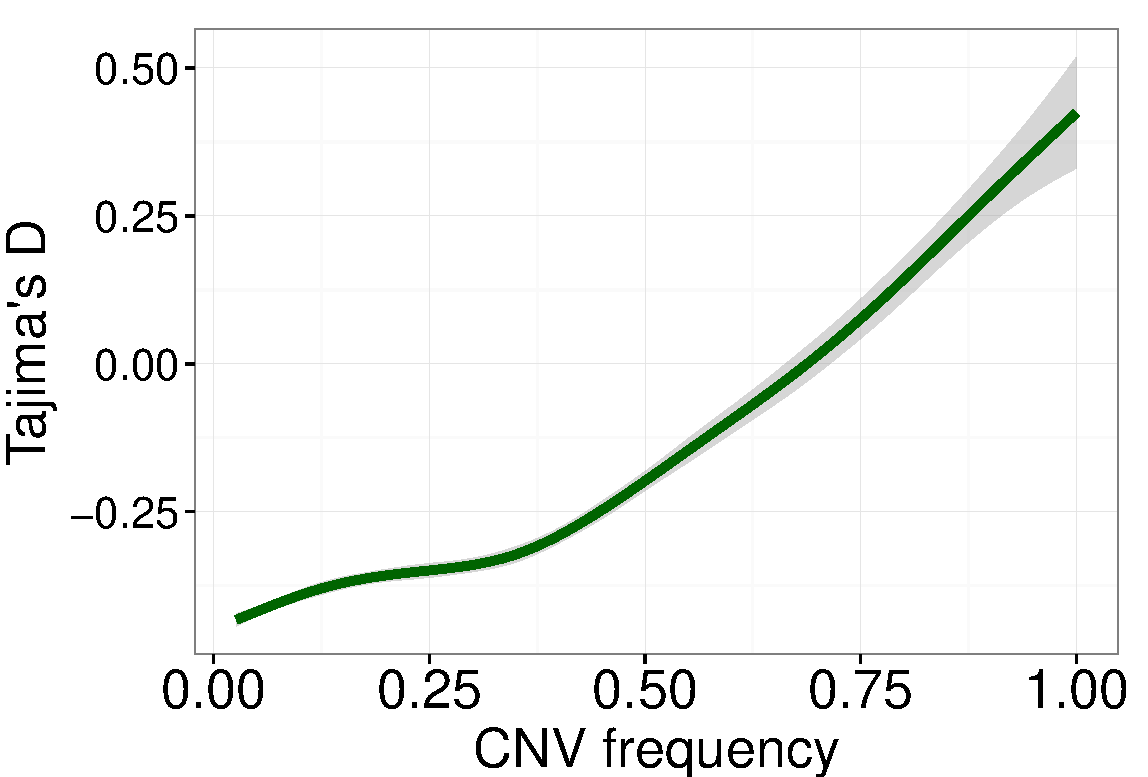
\includegraphics[width=0.45\linewidth]{figs/td_cnv.pdf}
\caption{The effect of copy number variation (CNV) on estimates of Tajima's D, a measure of the allele freqeuncy spectrum. In regions with no CNV, Tajima's D is negative consistent with population expansion. Tajima's D is inferred to be strongly postiive in regions with high-frequency CNVs, however, which could be (erroneously) interpreted as population decline or balancing selection.} 
\label{fig:tajd}
\end{SCfigure}
%

%\section*{Notes}
%
%\citep{peischl2015expansion} predict more u-shaped SFS in expanded pops, also more homozygous deleterious. this is seen in humans. Li's results in maize
%
%\citep{fu2014characteristics}
%``Indeed, a substantial amount of the higher density of deleterious alleles in EA individuals in the simulated data is attributable to weakly deleterious mutations $(|s| \approx 10^{-4})$''
%
%\citep{balick2013response} show weighted sum of the SFS can be used to differentiate recessive vs. not at deeteirous sites.
%
%\citep{lohmueller2014impact} 
%``Under a model where a mutation's effect on a trait is correlated with its effect on fitness, rare variants explain a greater portion of the additive genetic variance of the trait in a population that has recently expanded than in a population that did not recently expand. Further, when using a single-marker test, for a given false-positive rate and sample size, recent population growth decreases the expected number of significant associations with the trait relative to the number detected in a population that did not expand. However, in a model where there is no correlation between a mutation's effect on fitness and the effect on the trait, common variants account for much of the additive genetic variance, regardless of demography.''
%
%\citep{tennessen2012evolution} Shows vast majority of functionally important alleles rare, attributes to explosive population growth and weak purifying selection
%
%\citep{hufford2013genomic} \citep{hufford2012comparative}

%
%\begin{SCfigure}
%\includegraphics[width=0.45\linewidth]{joost_diversity.png}
%\caption{Changes in genetic diversity (represented as the effective number of ancestors) of the three primary maize heterotic groups (SS: stiff-stalk; NSS: non-stiff-stalk; IDT: iodent). Inbreds are divided into eras representing different time periods: 1:1930-1950; 2:1950-1980; 3:1985-1992. Figure from \citet{van2012historical}.} 
%\label{fig:diversity}
%\end{SCfigure}
%


%\begin{figure}
%\centering
%\includegraphics[width=0.7\linewidth]{yield.png}
%\caption{Blah} 
%\label{fig:piecewise}
%\end{figure}



\newpage
\bibliography{jri.bib}
\end{document}
